\documentclass[tikz,border=12pt]{standalone}
\usepackage[T1]{fontenc}
\usepackage{tgheros}
\usepackage{sfmath}
\usepackage{amsmath}
\usepackage{fontawesome5}
\usepackage{tikz}
\usetikzlibrary{arrows.meta,positioning,shapes.geometric,fit,backgrounds,calc}
\usepackage{xcolor}

\renewcommand{\familydefault}{\sfdefault}

% Professional Academic Systems Palette
\definecolor{crimsonaccent}{HTML}{990000}
\definecolor{slateblue}{HTML}{1E3A8A}
\definecolor{darkslate}{HTML}{0F172A}
\definecolor{bodytext}{HTML}{334155}
\definecolor{cardbg}{HTML}{FFFFFF}
\definecolor{subtlebg}{HTML}{F8FAFC}
\definecolor{bordergray}{HTML}{94A3B8}
\definecolor{lightborder}{HTML}{CBD5E1}

\begin{document}
\begin{tikzpicture}[
  font=\sffamily,
  >=Stealth,
  allactiveorgan/.style={
    draw=bordergray,
    fill=cardbg,
    rounded corners=0pt,
    line width=0.9pt,
    inner sep=6pt,
    align=center,
    text=darkslate
  },
  activearrow/.style={
    ->,
    line width=1.0pt,
    draw=crimsonaccent
  },
  allactivearrow/.style={
    ->,
    line width=0.9pt,
    draw=slateblue
  }
]

  % Top Banner: Stage 7 Governance
  \node[allactiveorgan, text width=7.4in, fill=subtlebg, draw=slateblue!60] (s7) {
    \textbf{\color{slateblue}\faIcon{balance-scale}\; 7. GOVERNANCE \& RELEASE GATE} $\cdot$ STPA Hazard Analysis $\cdot$ Bumpless Override $\cdot$ Defensible Release
  };

  % --- TOP ROW: Organs 1, 2, 3 ---
  \node[allactiveorgan, text width=2.22in, below=0.22in of s7.south west, anchor=north west] (s1) {
    \textbf{\color{slateblue}\faIcon{satellite-dish}\; 1. SENSING}\\
    {\footnotesize Photons / Voltages to DMA}\\
    {\scriptsize\color{bodytext}MIPI CSI-2 $\cdot$ SPI Bus Priority}
  };

  \node[allactiveorgan, text width=2.22in, right=0.37in of s1] (s2) {
    \textbf{\color{slateblue}\faIcon{eye}\; 2. PERCEPTION}\\
    {\footnotesize\mbox{ViT Encoders} $\cdot$ \mbox{DINOv2}}\\
    {\scriptsize\color{bodytext}3D Spatial Affordance Tokens}
  };

  \node[allactiveorgan, text width=2.22in, right=0.37in of s2] (s3) {
    \textbf{\color{slateblue}\faIcon{database}\; 3. MEMORY}\\
    {\footnotesize Temporal Belief $\cdot$ $SE(3)$ Trees}\\
    {\scriptsize\color{bodytext}JEPA / RSSM World Models}
  };

  % --- MIDDLE ROW: Organs 5, 4 ---
  \node[allactiveorgan, text width=3.51in, below=0.25in of s3.south east, anchor=north east] (s4) {
    \textbf{\color{slateblue}\faIcon{brain}\; 4. REASONING (System 2 $\cdot$ MPU)}\\
    {\footnotesize Vision-Language Foundation Models $\cdot$ 3D Goals}\\
    {\scriptsize\color{bodytext}Leases with Expiring TTL ($t_{\text{expire}}$)}
  };

  \node[allactiveorgan, text width=3.51in, left=0.38in of s4] (s5) {
    \textbf{\color{slateblue}\faIcon{network-wired}\; 5. PLANNING (System 1.5 $\cdot$ MPU/NPU)}\\
    {\footnotesize Diffusion Policies $\cdot$ \mbox{ACT Action Chunking}}\\
    {\scriptsize\color{bodytext}$H$-Step Action Horizons $\cdot$ $\mathcal{C}^2$ Jerk Continuity}
  };

  % --- LOWER ROW: Organ 6 ---
  \node[allactiveorgan, text width=7.4in, below=0.42in of s5.south west, anchor=north west, draw=crimsonaccent!80] (s6) {
    \textbf{\color{crimsonaccent}\faIcon{shield-alt}\; 6. REFLEX (System 1 $\cdot$ MCU)}\\
    {\footnotesize 1 kHz Real-Time Loop $\cdot$ Control Barrier Functions ($h(\mathbf{x}) \ge 0$) $\cdot$ Dynamic Stopping $d_{\text{stop}} \le d_{\text{clearance}} \cdot$ Veto ($u_t$)}
  };

  % --- PHYSICAL WORLD ROW ---
  \node[allactiveorgan, draw=crimsonaccent, fill=subtlebg, text width=7.4in, below=0.22in of s6.south west, anchor=north west] (world) {
    \textbf{\color{crimsonaccent}\faIcon{cogs}\; THE PHYSICAL WORLD ($W_t \to W_{t+1}$)} $\cdot$ Kinetic Momentum $\cdot$ Joule Heat $\cdot$ Friction $\cdot$ Collision Dynamics
  };

  % Proposal-Permission Boundary Line
  \coordinate (bleft) at ($(s6.north west) + (0, 0.22in)$);
  \coordinate (bright) at ($(s6.north east) + (0, 0.22in)$);
  \draw[dashed, line width=1.0pt, crimsonaccent] (bleft) -- (bright);
  \node[font=\sffamily\scriptsize\bfseries, fill=white, draw=crimsonaccent, rounded corners=0pt, inner sep=2.5pt, text=crimsonaccent] 
    at ($(bleft)!0.5!(bright)$) 
    {\faIcon{lock}\; THE PROPOSAL--PERMISSION PRIVILEGE BOUNDARY};

  % Connecting Arrows
  \draw[allactivearrow] (s1.east) -- (s2.west);
  \draw[allactivearrow] (s2.east) -- (s3.west);
  \draw[allactivearrow] (s3.south) -- (s3.south |- s4.north);
  \draw[allactivearrow] (s4.west) -- (s5.east);
  \draw[allactivearrow, dashed] (s5.south) -- (s5.south |- s6.north);
  \draw[activearrow] (s6.south) -- (world.north);

  % Closed-loop feedback from physical world back to sensing
  \draw[activearrow] (world.west) -- ++(-0.35in, 0) |- (s1.west) 
    node[pos=0.25, above, rotate=90, font=\sffamily\scriptsize\bfseries, text=crimsonaccent] {\faIcon{sync-alt}\; Endogenous Sensory Shift ($O_{t+1}$)};

\end{tikzpicture}
\end{document}
